% ====================================================================
% DESCRICAO-HARDWARE.TEX — Seção 3: Descrição de Hardware
% ====================================================================

\section{Descrição de Hardware}

Esta seção apresenta os componentes eletrônicos utilizados no protótipo, conforme
definido no esquemático do projeto (Monitoramento Ambiental — v1.0, EasyEDA, 2026-09-30),
com justificativas técnicas para cada escolha.

\begin{figure}[H]
    \centering
    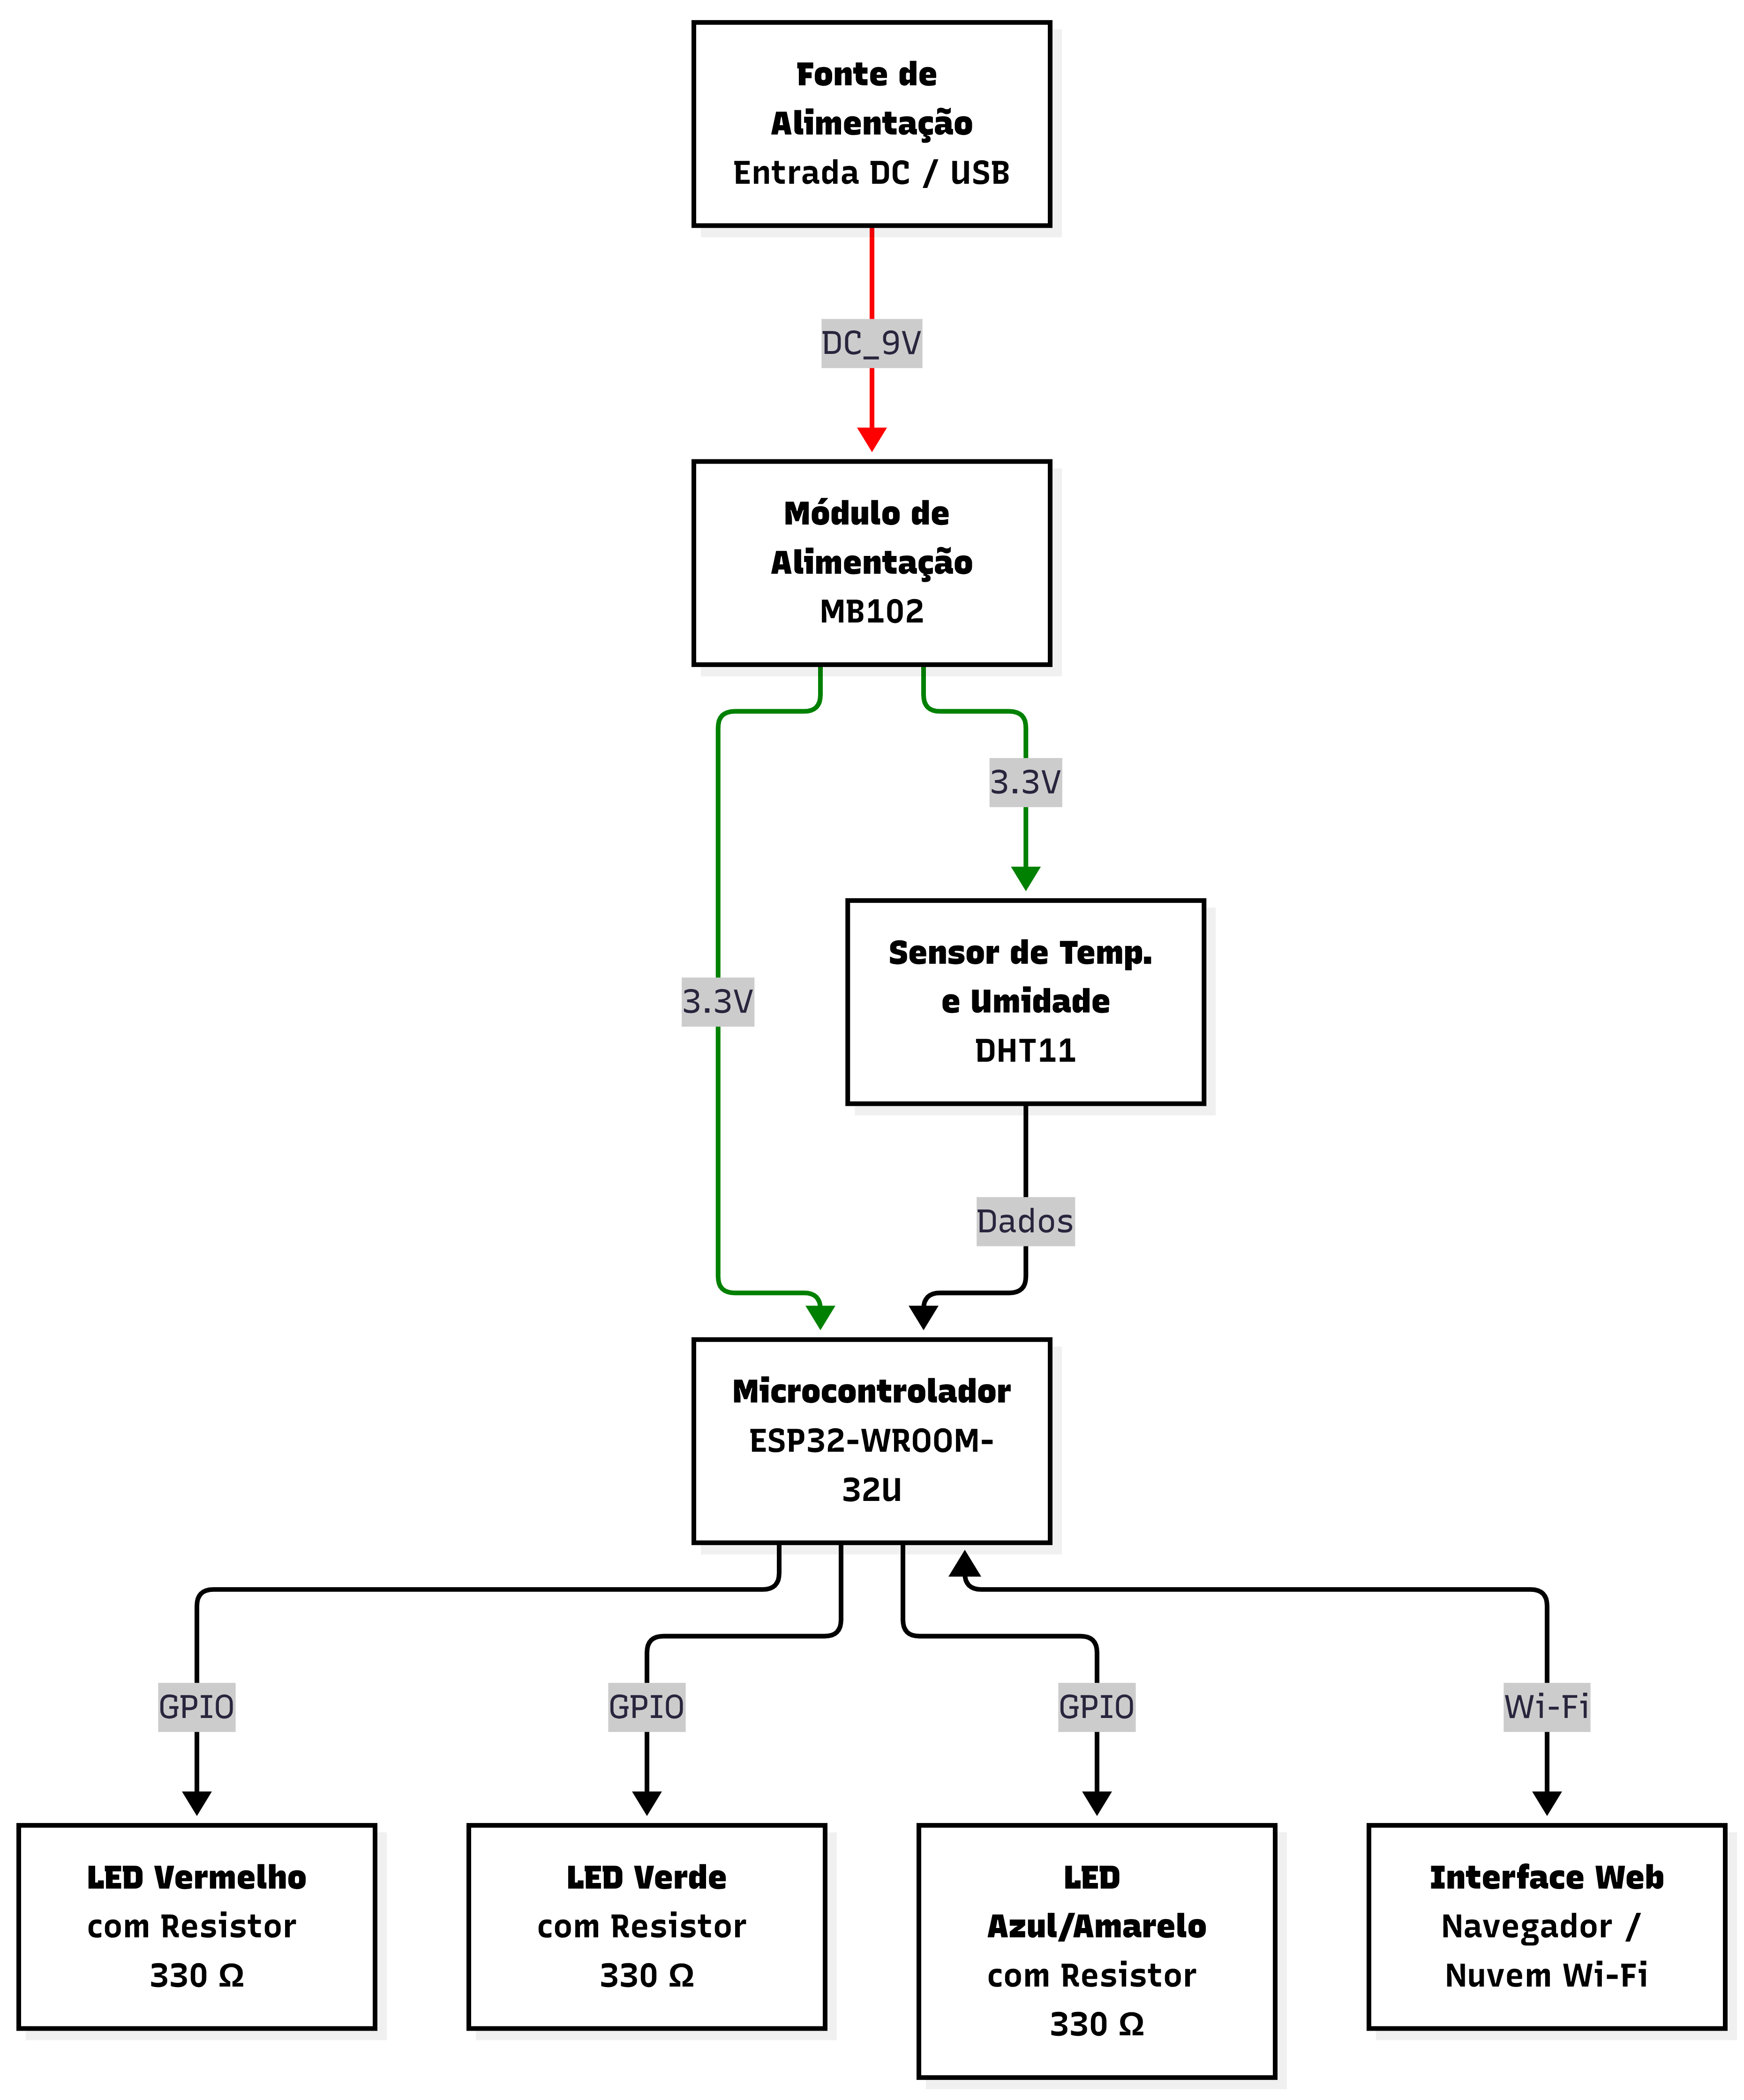
\includegraphics[width=\textwidth]{imag/diagrama-blocos.png}
    \caption{Diagrama de blocos do sistema de monitoramento ambiental.}
    \label{fig:diagrama-blocos}
\end{figure}

\begin{figure}[H]
    \centering
    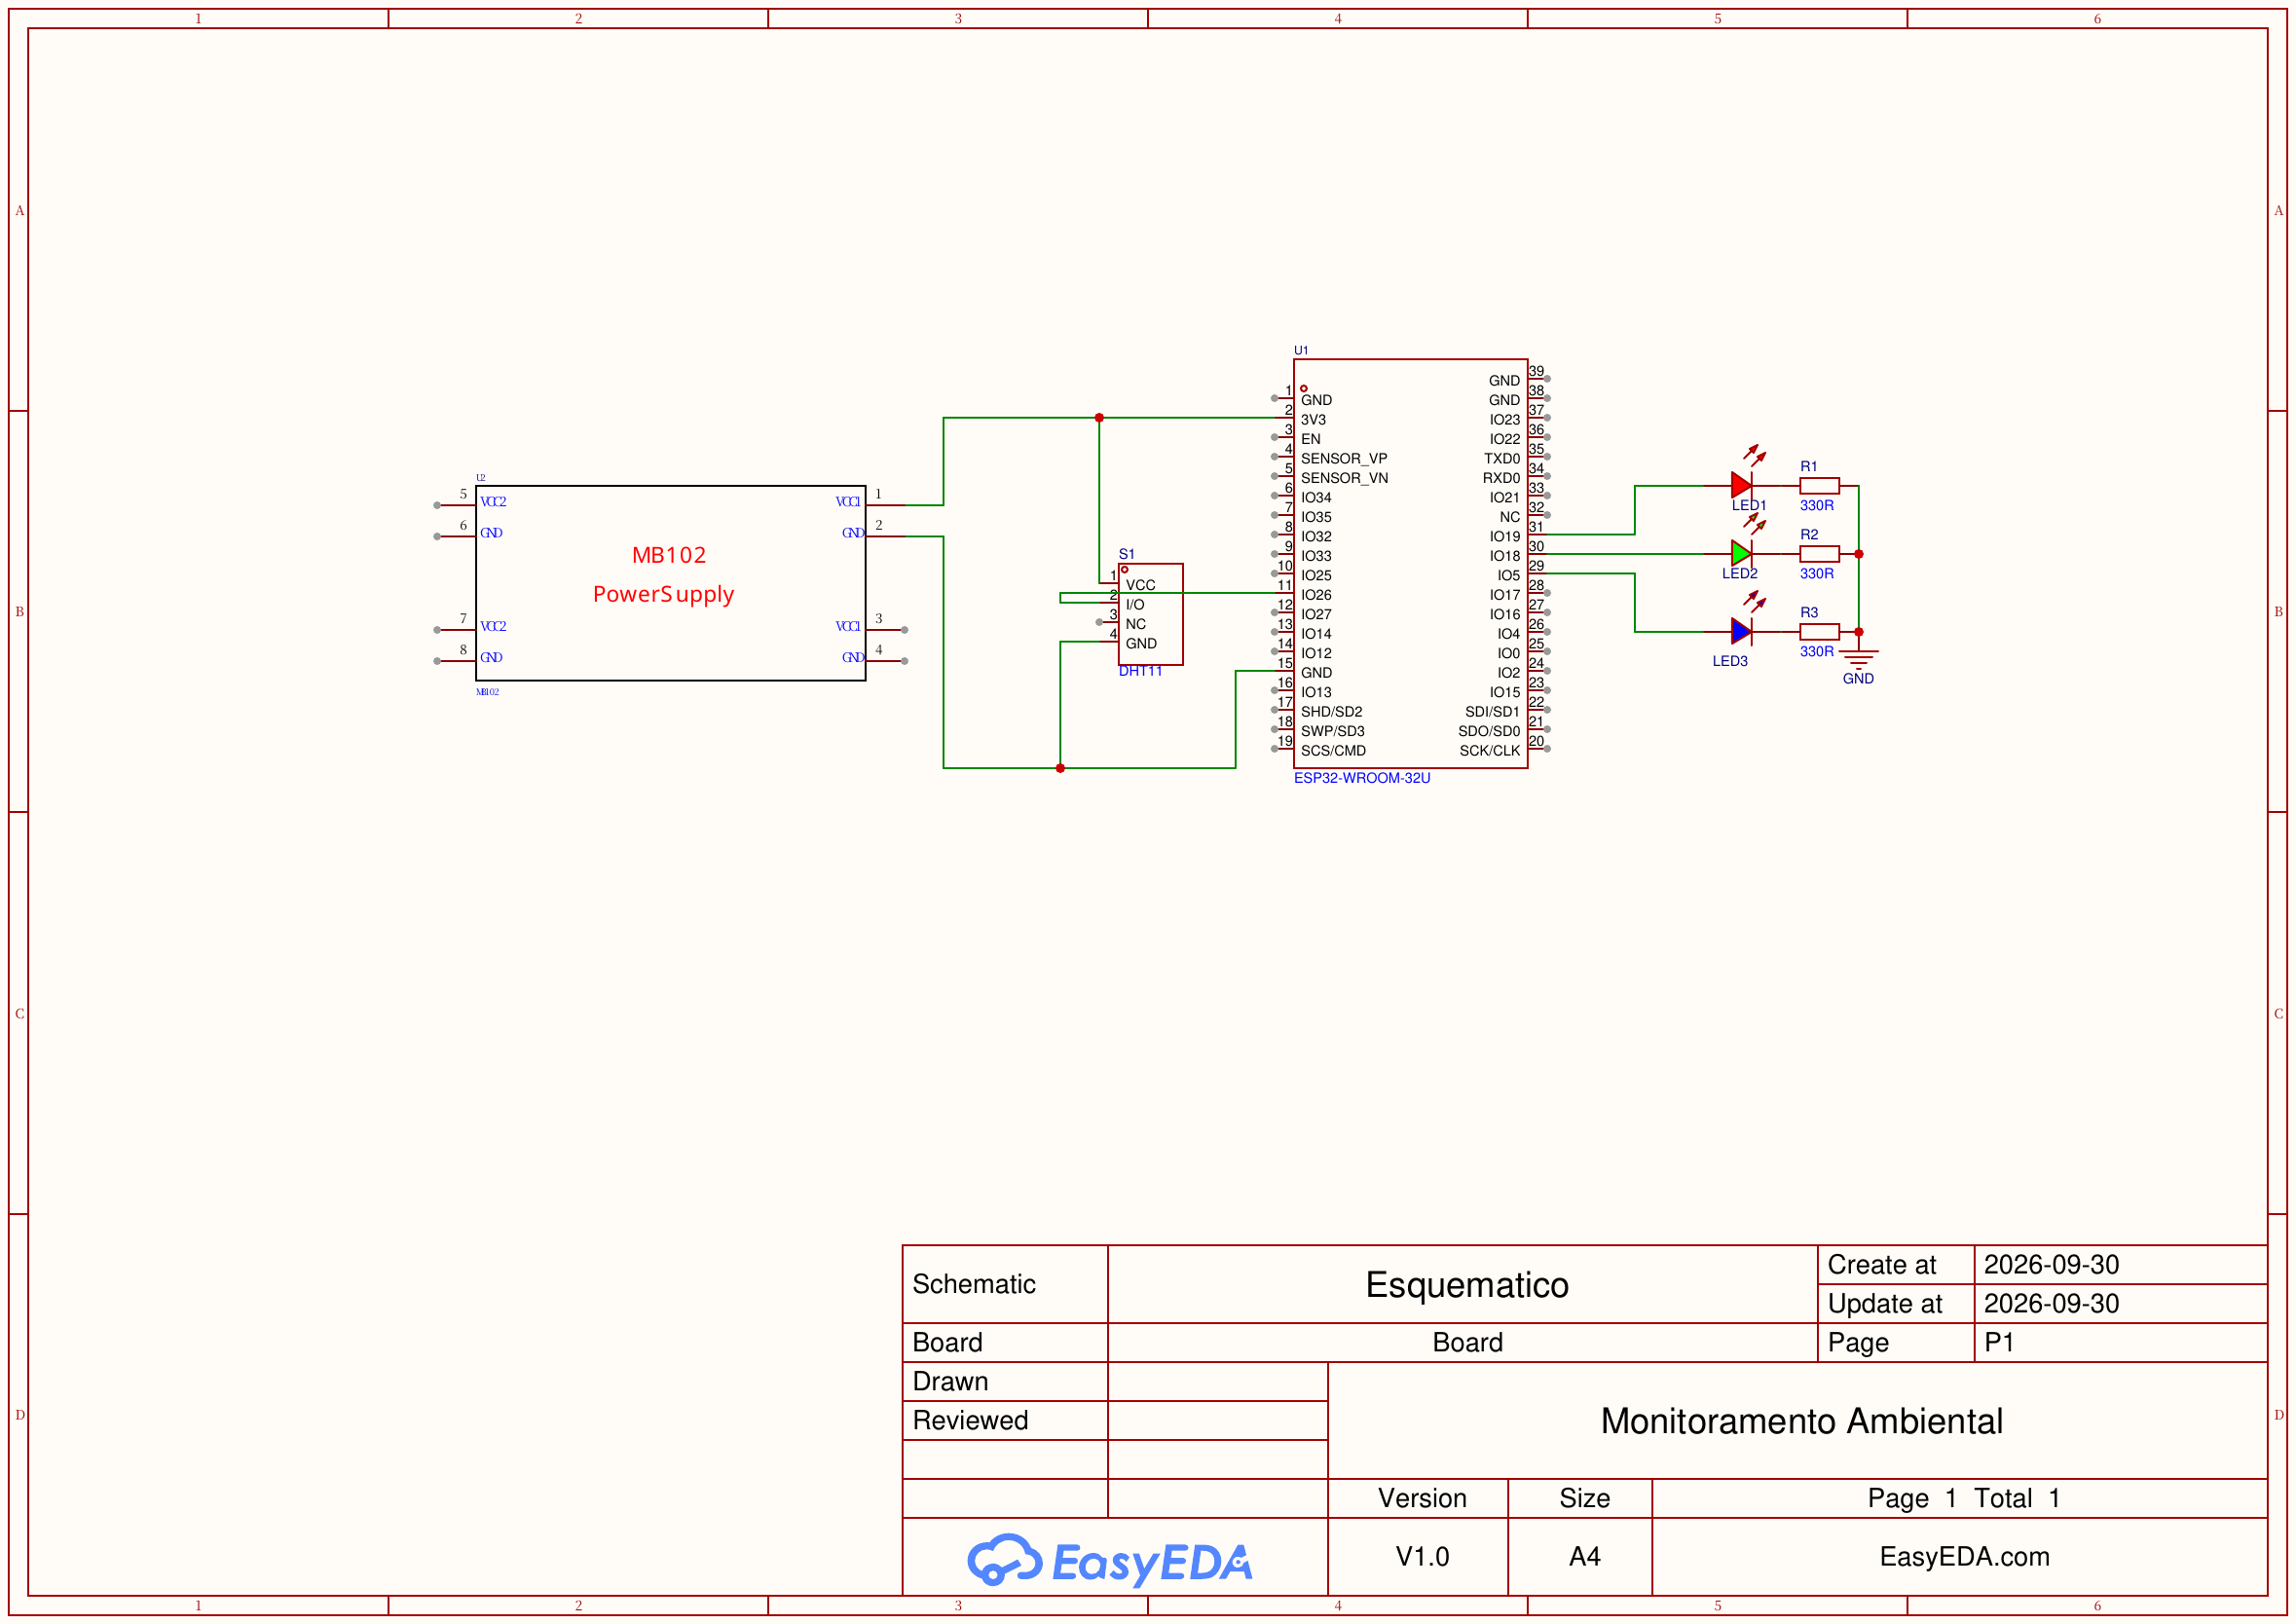
\includegraphics[width=\textwidth]{imag/esquematico.png}
    \caption{Esquemático do projeto de monitoramento ambiental (EasyEDA, 2026-09-30).}
    \label{fig:esquematico}
\end{figure}

% --------------------------------------------------------------------
\subsection{Microcontrolador — ESP32-WROOM-32U}
% --------------------------------------------------------------------

O microcontrolador selecionado foi o \textbf{ESP32-WROOM-32U} (referência U1 no esquemático),
módulo baseado no chip ESP32 da Espressif Systems.

As principais características que justificam sua escolha são:

\begin{itemize}
    \item \textbf{Conectividade Wi-Fi integrada (802.11 b/g/n):} permite a comunicação
    com a interface web sem necessidade de módulos externos, atendendo ao requisito RNF01.

    \item \textbf{Bluetooth integrado (BLE e Bluetooth Clássico):} recurso adicional
    disponível para expansões futuras.

    \item \textbf{Processador dual-core Xtensa LX6 a até 240 MHz:} capacidade de
    processamento suficiente para gerenciar a leitura do sensor, o servidor web e
    o controle dos LEDs simultaneamente.

    \item \textbf{GPIOs múltiplos:} o módulo disponibiliza mais de 30 pinos de I/O,
    suficientes para conexão do sensor DHT11 e dos três LEDs indicadores.

    \item \textbf{Suporte ao Arduino IDE e ESP-IDF:} facilidade de programação com
    ampla documentação e comunidade ativa.

    \item \textbf{Alimentação de 3,3 V:} compatível com a tensão fornecida pelo módulo
    MB102.
\end{itemize}

% --------------------------------------------------------------------
\subsection{Sensor de Temperatura e Umidade — DHT11}
% --------------------------------------------------------------------

O sensor utilizado é o \textbf{DHT11} (referência S1 no esquemático), um sensor digital
de temperatura e umidade de baixo custo amplamente utilizado em projetos embarcados.

Características técnicas relevantes:

\begin{itemize}
    \item \textbf{Faixa de medição de temperatura:} 0 °C a 50 °C, com precisão de ±2 °C.
    \item \textbf{Faixa de medição de umidade:} 20\% a 90\% UR, com precisão de ±5\% UR.
    \item \textbf{Interface digital single-wire:} comunicação por um único pino de dados,
    simplificando a conexão com o ESP32.
    \item \textbf{Tensão de operação:} 3,3 V a 5 V, compatível com o sistema.
    \item \textbf{Taxa de amostragem:} 1 leitura por segundo (1 Hz).
    \item \textbf{Pinagem:} VCC, I/O (dados), NC (não conectado) e GND.
\end{itemize}

O DHT11 foi selecionado por sua facilidade de integração com o ESP32, baixo custo
e suficiência para as condições ambientais internas típicas do projeto.

% --------------------------------------------------------------------
\subsection{LEDs Indicadores de Modo}
% --------------------------------------------------------------------

Três LEDs (LED1, LED2 e LED3 no esquemático) são utilizados para indicar visualmente
o modo de operação ativo do sistema, atendendo ao requisito RF07.

Cada LED está conectado em série com um resistor limitador de corrente de \textbf{330 $\Omega$}
(R1, R2 e R3), calculado para operar com a tensão de saída do ESP32 (3,3 V), garantindo
corrente segura para os LEDs (aproximadamente 5–10 mA).

A correspondência entre LEDs e modos de operação deve ser definida no firmware:

\begin{itemize}
    \item \textbf{LED1:} indicador do modo Ligado.
    \item \textbf{LED2:} indicador do modo Automático.
    \item \textbf{LED3:} indicador do modo Desligado.
\end{itemize}

% --------------------------------------------------------------------
\subsection{Módulo de Alimentação — MB102}
% --------------------------------------------------------------------

A alimentação do circuito é fornecida pelo \textbf{módulo MB102} (U2 no esquemático),
um regulador de tensão para protoboard/placa perfurada amplamente utilizado em
prototipagem.

Características:

\begin{itemize}
    \item \textbf{Entradas aceitas:} 6,5 V a 12 V via conector DC jack ou USB.
    \item \textbf{Saídas reguladas:} 3,3 V e 5 V selecionáveis por jumper, fornecidas
    nos dois barramentos VCC do circuito (VCC1 e VCC2).
    \item \textbf{Corrente máxima:} 700 mA por canal.
\end{itemize}

O módulo MB102 alimenta tanto o ESP32-WROOM-32U quanto o sensor DHT11,
simplificando o gerenciamento de energia do protótipo.

% --------------------------------------------------------------------
\subsection{Protoboard e Montagem}
% --------------------------------------------------------------------

Os componentes do protótipo serão montados em uma \textbf{protoboard comum},
possivelmente a de \textbf{830 pontos}, amplamente utilizada em prototipagem eletrônica.
A montagem seguirá o esquemático gerado no EasyEDA, respeitando as conexões entre
o ESP32, o DHT11, os LEDs com seus respectivos resistores e o módulo de alimentação MB102.
